Antes do projeto ser iniciado foi feito um planejamento do mesmo para que pudesse ter uma melhor organização, um controle do tempo e das entregas previstas.

\section{Cronograma}

O cronograma foi feito para guiar o projeto, principalmente para que as atividades pudessem ser cumpridas no tempo determinado. Ele foi elaborado usando a ferramenta Gantter.

\subsection{Cronograma - Primeira Entrega}

\FloatBarrier
\begin{figure}[!htpd]
		\centering
		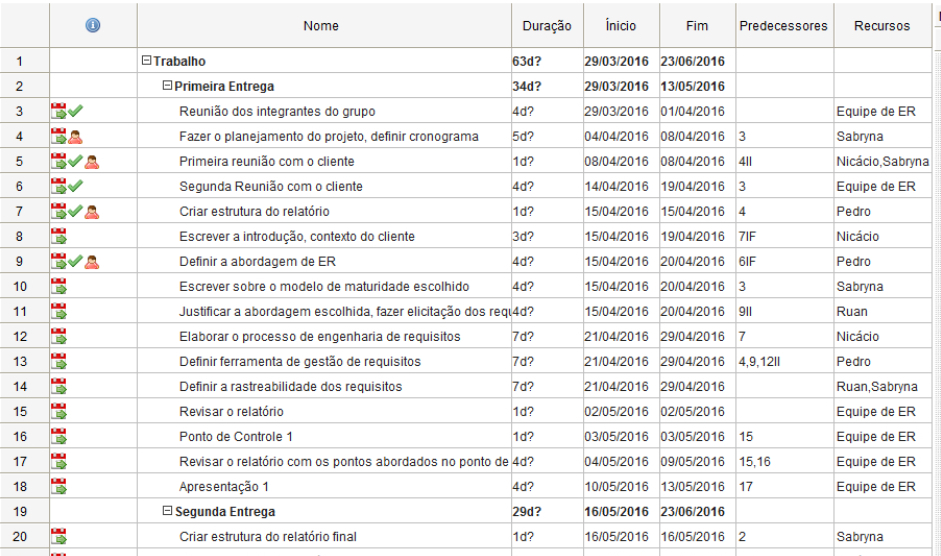
\includegraphics[scale=0.5]{figuras/cron1}
		\label{img:Cronograma - Primeira Entrega}
		\caption{Primeira Entrega}
\end{figure}
\FloatBarrier

\subsection{Cronograma - Segunda Entrega}

\FloatBarrier
\begin{figure}[!htpd]
		\centering
		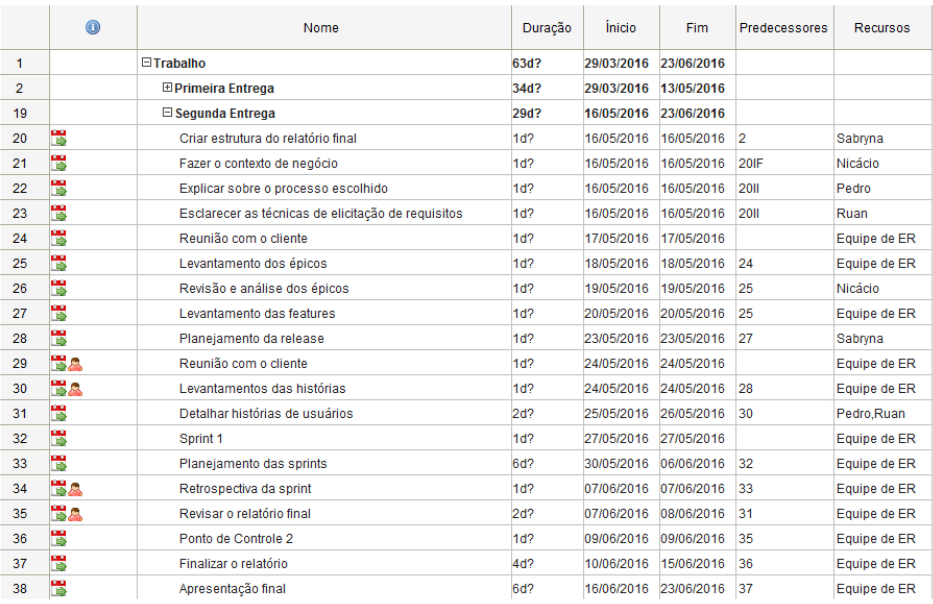
\includegraphics[scale=0.5]{figuras/cron2}
		\label{img:Cronograma - Segunda Entrega}
		\caption{Segunda Entrega}
\end{figure}
\FloatBarrier
